% This is samplepaper.tex, a sample chapter demonstrating the
% LLNCS macro package for Springer Computer Science proceedings;
% Version 2.20 of 2017/10/04
%
\documentclass[runningheads]{llncs}
%
\usepackage{graphicx}
% Used for displaying a sample figure. If possible, figure files should
% be included in EPS format.
%  
% If you use the hyperref package, please uncomment the following line
% to display URLs in blue roman font according to Springer's eBook style:
% \renewcommand\UrlFont{\color{blue}\rmfamily}
\usepackage{amsmath}

\usepackage{booktabs}
\usepackage{multirow}
\usepackage{makecell}

\newcommand{\hdrule}{\midrule[\heavyrulewidth]}
\newcommand{\argmin}{\mathop{\mathrm{arg\,min}}}
\newcommand{\beginsupplement}{%
        \setcounter{table}{0}
        \renewcommand{\thetable}{S\arabic{table}}%
        \setcounter{figure}{0}
        \renewcommand{\thefigure}{S\arabic{figure}}%
        \setcounter{section}{0}
        \renewcommand{\thesection}{S\arabic{section}}%
        \setcounter{equation}{0}
        \renewcommand{\theequation}{S\arabic{equation}}%
     }

\begin{document}
%
\title{Learning Deeply Enriched Representations of Longitudinal Imaging-Genetic Data to Predict Alzheimer's Disease Progression}
\author{}
\institute{}

% \author{First Author\inst{1}\orcidID{0000-1111-2222-3333} \and
% Second Author\inst{2,3}\orcidID{1111-2222-3333-4444} \and
% Third Author\inst{3}\orcidID{2222--3333-4444-5555}}
%
% \authorrunning{F. Author et al.}
% First names are abbreviated in the running head.
% If there are more than two authors, 'et al.' is used.
%
% \institute{Princeton University, Princeton NJ 08544, USA \and
% Springer Heidelberg, Tiergartenstr. 17, 69121 Heidelberg, Germany
% \email{lncs@springer.com}\\
% \url{http://www.springer.com/gp/computer-science/lncs} \and
% ABC Institute, Rupert-Karls-University Heidelberg, Heidelberg, Germany\\
% \email{\{abc,lncs\}@uni-heidelberg.de}}
%
\maketitle              % typeset the header of the contribution
%
\begin{abstract}
Alzheimer’s Disease (AD) is a progressive memory disorder that causes irreversible cognitive decline. Early diagnosis is imperative to prevent the progression of AD and many biomarker analysis models have been presented to detect the disease in its early stages. However, these models often lack reliability due to their failure to integrate longitudinal (dynamic) phenotypic data with (static) genetic data, and/or to fully utilize both labeled and unlabeled samples.
% deal with the missing data in the incomplete temporal neuroimaging records. 
To overcome these difficulties, we propose a semi-supervised enrichment learning method to learn the fixed-length vectorial representation of dynamic data for each participant. 
% Our enrichment model combines a novel long short-term memory (LSTM) autoencoder and a deep neural network which learns the vectorial representation of dynamic data from the available labeled samples. 
Armed with the enriched representation in fixed-length vector format, the static data can be readily integrated with the dynamic data.
% Our enrichment model is the ensemble of the novel long short-term memory (LSTM) autoencoder and the deep neural networks which is designed to handle multi-modal information and utilize the labeled and unlabeled samples both. 
We have applied our new method on the Alzheimer's Disease Neuroimaging Initiative (ADNI) cohort and achieved 75\% accuracy on multiclass AD progression prediction one year in advance. In addition to the improved prediction performance when compared against several widely used machine learning algorithms, the proposed model identifies the most relevant disease biomarkers.

% \keywords{First keyword  \and Second keyword \and Another keyword.}
\end{abstract}

% Manuscripts should be up to 8-pages (text, figures and tables) plus up to 2 pages of references.
% The MICCAI Conference review process will be double-blind, i.e. the names of the authors will be hidden from the Area Chairs and Reviewers, and the names of Reviewers and Area Chairs will not be revealed to the authors

% should reduce 1.3 pages, intro -> 0.2 
\iffalse
Mild cognitive impairment (MCI) is a transitional stage between age-related cognitive decline and Alzheimer’s disease (AD). For the effective treatment of AD, it would be important to identify MCI patients at high risk for conversion to AD. 
The novel characteristics of the methods for learning the biomarkers are as follows: 1) We used a semi-supervised learning method (low density separation) for the construction of MRI biomarker as opposed to more typical supervised methods; 2)
4) We constructed the aggregate biomarker by first learning a separate MRI biomarker and then combining it with age and cognitive measures about the MCI subjects at the baseline by applying a random forest classifier.
Alzheimer’s disease (AD), a common form of dementia, occurs most frequently in aged population. More than 30 million people worldwide suffer from AD and, due to the increasing life expectancy, this number is expected to triple by 2050 (The projected effect of risk factor reduction on Alzheimer's disease prevalence, Barnes DE).
Because of the dramatic increase in the prevalence of AD, the identification of effective biomarkers for the early diagnosis and treatment of AD in individuals at high risk to develop the disease is crucial.
Mild cognitive impairment (MCI) is a transitional stage between age-related cognitive decline and AD, and the earliest clinically detectable stage of progression towards dementia or AD (Neuropathologic alterations in mild cognitive impairment: a review, Markesbery WR). 
AD pathology has been therefore hypothesized to be detectable using neuroimaging techniques.(Neuropathologic alterations in mild cognitive impairment: a review, Markesbery WR)
Among different neuroimaging modalities, MRI has attracted a significant interest in AD related studies because of its completely non-invasive nature, high availability, high spatial resolution and good contrast between different soft tissues.
Clearly, predicting this disease in the early stages and preventing it from progressing is of great importance.
The diagnosis of Alzheimer’s disease (AD) requires a variety of medical tests, which leads to huge amounts of multivariate heterogeneous data. It can be difficult and exhausting to manually compare, visualize, and analyze this data due to the heterogeneous nature of medical tests; therefore, an efficient approach for accurate prediction of the condition of the brain through the classification of magnetic resonance imaging (MRI) images is greatly beneficial and yet very challenging. In this paper, a novel approach is proposed for the diagnosis of very early stages of AD through an efficient classification of brain MRI images
Next, using a small set of labeled training data,
The reason that early diagnosis of AD is of great importance is that the clinical therapies given to patients are much more effective in slowing down disease progression and helping preserve some cognitive functions of the brain if the patients are in the early stages of their disease.
In this paper, we propose a novel method for a high-level latent and shared feature representation from neuroimaging modalities via deep learning. 
Furthermore, fusing the complementary information from multiple modalities helps enhance the diagnostic accuracy[Identification of conversion from mild cognitive impairment to Alzheimer's disease using multivariate predictors.; Multivariate examination of brain abnormality using both structural and functional MRI.]
To this end, many researchers have devoted their efforts to find biomarkers and develop a computer-aided system, with which we can effectively predict or diagnose the diseases.
In a semi-supervised method, feature vectors from unlabeled data are also used in the learning process in addition to the labels and feature vectors from the labeled ones.
\fi

\section{Introduction}
% Why our model is good? : (1) Semi-supervised learning -> Our model can learn from labeled/unlabeled samples BOTH. (2) Learn temporal trends from the time series with missing records (MRI imagings are captured inconsistently (the number of records/the time points of records are different) from the participants). (3) Combine the multi-modal (genotypic modality (SNPs, static) + phenotypic (neuroimagings, dynamic) modality) data with two Autoencoders: one for static, another for time series.
% Find the related works with the lack of above advantages of our model.
\iffalse
For AD progression prediction using longitudinal phenotypic markers, the input imaging features are a set of matrices X = {X1, X2, . . . , XT } ∈ Rd×n×T corresponding to the measurements at T consecutive time points, where Xt is the phenotypic measurements for a certain type of imaging markers, such as voxel-based morphometry (VBM) markers (see details in Section 3) used in this study, at time t (1 ≤ t ≤ T ).
\fi

\section{The Dataset and Problem Formalization}
\subsection{Datasets}
We obtained the data used in this experiment from the ADNI database~\cite{risacher2010longitudinal}. We downloaded 1.5 T MRI scans, single nucleotide polymorphisms (SNPs), and demographic information (age and gender) of 821 ADNI-1 participants. For the SNPs data, the quality control steps discussed in~\cite{shen2010whole} were followed, and 1223 SNPs for each participant are extracted. We performed voxel-based morphometry (VBM) and FreeSurfer (FS) on the MRI data following~\cite{risacher2010longitudinal} and extracted mean modulated gray matter measures for 90 target regions of interest. We also downloaded the longitudinal scores of the participants in five independent cognitive assessments including Alzheimer’s Disease Assessment Scale (ADAS), Mini-Mental State Examination (MMSE), Fluency test (FLU), Rey’s Auditory Verbal Learning Test (RAVLT) and Trail making test (TRAILS). 
% We also downloaded the longitudinal scores of the participants in five independent cognitive assessments including Alzheimer’s Disease Assessment Scale (ADAS)~\cite{rosen1984new}, Mini-Mental State Examination (MMSE)~\cite{tombaugh1992mini}, Fluency test (FLU)~\cite{ruff1987ruff}, Rey’s Auditory Verbal Learning Test (RAVLT)~\cite{moradi2017rey} and Trail making test (TRAILS)~\cite{reitan1958validity}. 
% Details about these cognitive assessments are available in the ADNI procedure manuals\footnote{http://adni.loni.usc.edu/wp-content/uploads/2010/09/ADNI\_GeneralProceduresManual.pdf}. 
In this analysis, the time points for both imaging records and cognitive assessments include baseline (BL), month 6 (M6), month 12 (M12), month 18 (M18), and month 24 (M24). We use the diagnosis at month 36 (M36) in Alzheimer's disease (AD), mild cognitive impairment (MCI), and healthy control(HC) as predictive target in our studies. The participants with no missing SNPs, demographic information, and AD diagnosis at M36 were included, providing a set of 379 subjects (104 AD, 115 MCI, 160 HC). The studied cohort includes 231 male and 148 female participants, and the average age is 75.35.
% Why multi class?

In the following pages, we denote a vector as a bold lower case letter, and a matrix as a bold upper case letter. For the arbitrary matrix $\mathbf{X}$, $[\mathbf{X}]^r$, $[\mathbf{X}]_c$, $[\mathbf{X}]^r_c$ denotes the $r$-th row, $c$-th column, an element of $r$-th row and $c$-th column respectively. We use $i$ and $j$ to index the participant and record respectively. We describe the records of the $i$-th participant as $\mathcal{X}_i = \{\mathbf{x}_i^b, \mathbf{x}_i^s, \mathbf{X}_i, \mathbf{M}_i, \mathbf{t}_i\}$. $\mathbf{x}_i^b \in \Re^{D_b}$ is a vector of basic demographic information (age and gender, $D_b = 2$), $\mathbf{x}_i^s \in \Re^{D_s}$ is a vector of SNPs ($D_s = 1223$), and $\mathbf{X}_i = [\mathbf{x}_i^1; \mathbf{x}_i^2; \cdots; \mathbf{x}_i^{n_i}] \in \Re^{n_i \times D_l}$ are the longitudinal records collected across the $n_i$ time points. $\mathbf{M}_i = [\mathbf{m}_i^1; \mathbf{m}_i^2; \cdots; \mathbf{m}_i^{n_i}] \in \{1, 0\}^{n_i \times D_l}$ are the binary masks of longitudinal records $\mathbf{X}_i$, where 1 and 0 indicates the observed and unobserved entry. Each longitudinal record at the $j$-th time point $\mathbf{x}_i^j$ ($1 \leq j \leq n_i$) is the concatenation of multi-modal neuroimagings and cognitive assessments, such that $\mathbf{x}_i^j = $ $[\mathbf{x}_{i,VBM}^j$, $\mathbf{x}_{i,FS}^j,$ $\mathbf{x}_{i,ADAS}^j,$ $\mathbf{x}_{i,MMSE}^j,$ $\mathbf{x}_{i,FLU}^j,$ $\mathbf{x}_{i,RAVLT}^j,$ $\mathbf{x}_{i,TRAILS}^j] \in \Re^{D_l}$, and the missing records are filled with the constant $-1$. $\mathbf{t}_i = [t_i^1; t_i^2; \cdots; t_i^{n_i}] \in \Re^{n_i}$ are the time stamps of $n_i$ records. The target label $\mathbf{y}_i \in \Re^{D_y}$ of the $i$-th participant is given for training if that participant is in training set, such that $i \in \Omega_{train}$. 
% The target label is one-hot encoded, such that $[1, 0, 0]$, $[0, 1, 0]$, and $[0, 0, 1]$ represent AD, MCI, and HC respectively. 
The input and output of the proposed model is described in Fig.~\ref{fig: final-inputs}.
\begin{figure}
    \centering
    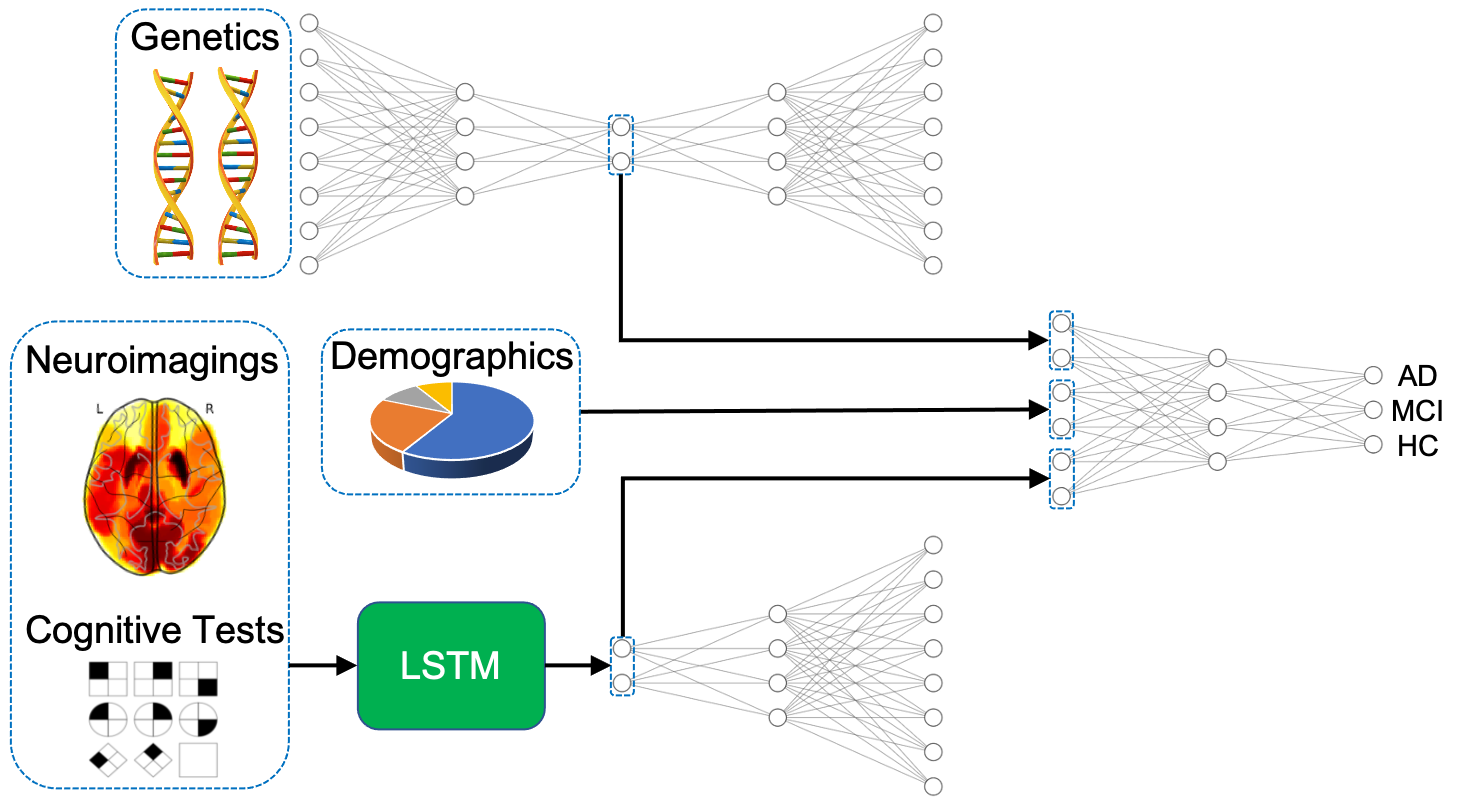
\includegraphics[width=0.95\textwidth]{images/final-inputs.png}
    \caption{Armed with the enriched representations of dynamic and static data, we can fully utilize the information in the dataset. 
    % The demographic information is provided without enrichment, as it's dimensionality is relatively small.
    } \label{fig: final-inputs}
\end{figure}

\subsection{Enrichment and Objective Formulation}
\subsubsection{Static Data Enrichment}
We leverage the autoencoder~\cite{kramer1991nonlinear} to learn the enriched representation of genotypic biomarkers. The autoencoder consists of two deep neural networks: an encoder $\phi_{SNP}: \Re^{D_s} \mapsto \Re^{d_s}$ that encodes a vector of SNPs into the enriched representation such that $\phi_{SNP}(\mathbf{x}_i^s;\ \theta^s_{E}) = \mathbf{z}_i^s$, and an decoder $\psi_{SNP}: \Re^{d_s} \mapsto \Re^{D_s}$ that decodes the enriched representation into the reconstructed vector of SNPs such that $\psi_{SNP}(\mathbf{z}_i^s;\ \theta^s_{D}) = \tilde{\mathbf{x}}_i^s$. $\theta_{E}^s$ and $\theta_{D}^s$ is the set of trainable weights matrices and bias vectors for the encoder and decoder respectively. 
% The deep neural network is defined as the $K$ consecutive fully connected layers where the output of the $k$-th layer is:
% \begin{equation}
%     \mathbf{h}_k = \sigma(\mathbf{h}_{k-1}\mathbf{W}_k + \mathbf{b}_k),
% \end{equation}
% where $\sigma$ is an activation function.
% The input $\mathbf{h}_0$ of the network is then forwarded to the last layer $\mathbf{h}_K = \tilde{\mathbf{x}}_i^s$, which is the output of the network. 
The encoded representation $\mathbf{z}_i^s$ preserves as much information as possible while removing the redundant noises in SNPs $\mathbf{x}_i^s$ by updating $\theta_{E}^s$ or $\theta_{D}^s$ to minimize the following reconstruction loss:
\begin{equation}
    \mathcal{L}_{static}(\mathbf{x}_i^s, \tilde{\mathbf{x}}_i^s;\ \theta_{E}^s, \theta_{D}^s) = \left\|\mathbf{x}_i^s - \tilde{\mathbf{x}}_i^s\right\|_F^2,
\end{equation}
where squared Frobenious norm $\| \cdot \|_F^2$ is summation of all the entries squared.

% then combining it with age and cognitive measures.
% Our models summarizes the dynamic and static data into a fixed-length vectorial representation.
% We use Long Short Term Memory (LSTM) architecture to learn the fixed-length vectorial abstract representation summarizing the incomplete time series with varying length and uneven time intervals.
% [In this section, we describe the semi-supervised AutoEncoder (AE) structure to learn a fixed-length vectorial representation for each patient's longitudinal records with varying length. The proposed AE is a composite model of three components. The encoder $\phi_E$ learns an abstract enriched representation of the input time series data. The decoder $\phi_D$ learns the reconstruction system to estimate the original data from the enriched representation. The predictor $\phi_P$ learns the prediction system to estimate the target labels from the enriched representation.].

\subsubsection{Dynamic Data Enrichment}
LSTM encoder $\phi_{dynamic}: \Re^{n_i \times (2 D_l + 1)} \mapsto \Re^{d_l}$ summarizes the longitudinal records $\mathbf{X}_i$ in the fixed-length vector $\mathbf{z}_i^l$. The time stamp of each record is crucial in learning the temporal relation (e.g. temporal locality) between records, and the pattern of missing entries may help the encoder to interpret the input. Thus we provide the concatenation of longitudinal records, masks, and time stamps, $[\mathbf{X}_i, \mathbf{M}_i, \mathbf{t}_i] = [\hat{\mathbf{x}}_i^1; \hat{\mathbf{x}}_i^2; \cdots; \hat{\mathbf{x}}_i^{n_i}] = \hat{\mathbf{X}}_i \in \Re^{n_i \times (2 D_l + 1)}$, as an input of the LSTM encoder such that $\phi_{dynamic}(\mathbf{X}_i, \mathbf{M}_i, \mathbf{t}_i;\ \theta_{E}^l) = \mathbf{z}_i^l$. 

The concatenated longitudinal record at the $j$-th time step $\hat{\mathbf{x}}_i^j$ ($1 \leq j \leq n_i$) is processed by the following LSTM architecture~\cite{yu2019review}:
\begin{equation}
    \mathbf{k}^j_i = \sigma(\hat{\mathbf{x}}^j_i \mathbf{W}_{xk} + \mathbf{h}_i^{j-1} \mathbf{W}_{hk} + \mathbf{c}_i^{j-1} \mathbf{W}_{ck} + \mathbf{b}_k),
\end{equation}
\begin{equation}
    \mathbf{f}^j_i = \sigma(\hat{\mathbf{x}}^j_i \mathbf{W}_{xf} + \mathbf{h}^{j-1}_i \mathbf{W}_{hf} + \mathbf{c}^{j-1}_i \mathbf{W}_{cf} + \mathbf{b}_f),
\end{equation}
\begin{equation}
    \mathbf{c}^j_i = \mathbf{f}^j_i \odot \mathbf{c}^{j-1}_i + \mathbf{k}^j_i \odot \operatorname{tanh}(\hat{\mathbf{x}}_i^j \mathbf{W}_{xc} + \mathbf{h}^{j - 1}_i \mathbf{W}_{hc} + \mathbf{b}_c),
\end{equation}
\begin{equation}
    \mathbf{o}^j_i = \sigma(\hat{\mathbf{x}}_i^j \mathbf{W}_{xo} + \mathbf{h}^{j-1}_i \mathbf{W}_{ho} + \mathbf{c}^j_i \mathbf{W}_{co} + \mathbf{b}_o),
\end{equation}
\begin{equation}
    \mathbf{h}^j_i = \mathbf{o}^j_i \odot \operatorname{tanh}(\mathbf{c}^j_i),
\end{equation}
% \begin{equation}
% \begin{aligned}
%     \mathbf{k}^j_i = \sigma(\hat{\mathbf{x}}^j_i \mathbf{W}_{xk} + \mathbf{h}_i^{j-1} \mathbf{W}_{hk} + \mathbf{c}_i^{j-1} \mathbf{W}_{ck} + \mathbf{b}_k),\ \mathbf{f}^j_i = \sigma(\hat{\mathbf{x}}^j_i \mathbf{W}_{xf} + \mathbf{h}^{j-1}_i \mathbf{W}_{hf} + \mathbf{c}^{j-1}_i \mathbf{W}_{cf} + \mathbf{b}_f),
% \end{aligned}
% \end{equation}
where $\mathbf{k}^j_i$, $\mathbf{o}^j_i$, $\mathbf{f}^j_i$ are the input, output, and forget gate of the $j$-th time step respectively. \{$\mathbf{W}_{xk}$, $\mathbf{W}_{hk}$, $\mathbf{W}_{ck}$, $\mathbf{W}_{xf}$, $\mathbf{W}_{hf}$, $\mathbf{W}_{cf}$, $\mathbf{W}_{xc}$, $\mathbf{W}_{hc}$, $\mathbf{W}_{xo}$, $\mathbf{W}_{ho}$, $\mathbf{W}_{co}$\} $\subset \mathbf{\theta}_{E}^l$ are trainable weight matrices and $\{\mathbf{b}_k, \mathbf{b}_f, \mathbf{b}_c, \mathbf{b}_o\} \subset \mathbf{\theta}_{E}^l$ are trainable bias vectors. $\mathbf{c}_i^j$ and $\mathbf{h}_i^j$ denote the cell state and hidden representation. The hidden representation $\mathbf{h}_i^{n_i}$ at the last time step $n_i$ represents a summary of \emph{whole} longitudinal records $\hat{\mathbf{X}}_i$, such that $\mathbf{h}_i^{n_i} = \mathbf{z}_i^l \in \Re^{d_l}$. Since the hidden representation at the $j$-th time point aims to summarize the records from the first time step to the $j$-th time step, it refers to the cell state $\mathbf{c}_i^j$ containing information about the previous records. The cell state $\mathbf{c}_i^j$ is guided by the input gate $\mathbf{k}_i^j$ and forget gate $\mathbf{f}_i^j$, which control how much information from the previous step should be preserved, therefore cell state $\mathbf{c}_i^j$ enables the hidden representation $\mathbf{h}_i^j$ to learn long term dependencies. 
% For example, the LSTM encoder can capture the cognitive decline from the temporal trends in the scores of cognitive assessments.

% (RNN)~\cite{medsker2001recurrent}
We propose a decoder for dynamic data enrichment with a fully connected layers instead of another LSTM. A previous study~\cite{srivastava2015unsupervised} that attempted to enrich longitudinal records with a recurrent neural network, did so by using RNNs for both the encoder and decoder, where the output (reconstructed record) of the decoder at each time step depends on the output at the previous time step. However, since no additional information is provided to the decoder other than a time stamp and a learned representation that is no longer longitudinal, there should not be dependency between the outputs of the decoder. Therefore the decoder $\psi_{dynamic}:\Re^{d_l + 1} \mapsto \Re^{D_l}$ should be able to reconstruct the $j$-th record $\mathbf{x}_i^j$ given time stamp $t_i^j$ without any additional information, such that $\psi_{dynamic}(\mathbf{z}_i^l, t^j_i;\ \theta^l_{D}) = \tilde{\mathbf{x}}_i^j \approx \mathbf{x}_i^j$. This architecture, to the best of our knowledge, has not yet been proposed. We update $\theta^l_{E}$ and $\theta^l_{D}$ to minimize the error between the reconstructed and original records for the observed entries defined as: 
% indicated by the mask $\mathbf{M}_i$:
\begin{equation}
    \mathcal{L}_{dynamic}(\mathbf{X}_i, \tilde{\mathbf{X}}_i, \mathbf{M}_i;\ 
    \theta^l_{E}, \theta^l_{D}) = \frac{\left\| (\tilde{\mathbf{X}}_i
- \mathbf{X}_i) \odot \mathbf{M}_i
\right\|_F^2}{\sum_{q=1}^{D_l}\sum_{j=1}^{n_i}[\mathbf{M}_i]^j_q},
\end{equation}
where $\tilde{\mathbf{X}}_i \in \Re^{n_i \times D_l}$ is the stack of reconstructed $n_i$ records of $i$-th participant. 
% Why decoder is not RNN? Think of what is input for encoder and decoder. Because there is no information is additionally provided, current prediction depends on previous prediction does not make sense. The enriched representation is the fixed-length vector which is not longitudinal records anymore.

% Although the enriched representation is learned from a few of observations, it represents the whole temporal dimension of timeseries.
% Given the enriched representation $\mathbf{z}_i^l$, the decoder tries to estimate the function of time $\psi_{dynamic}(t; \mathbf{z}_i^l)$ to reconstruct the state of biomarker representation in temporal dimension.

\subsubsection{Prediction and Loss Function}
From the enriched representations $\mathbf{z}_i^l$ and $\mathbf{z}_i^s$ of dynamic and static data, another fully connected layer $\psi_{pred}: \Re^{(d_s + d_l + D_b)}  \mapsto \Re^{D_y}$ predicts the target label $\mathbf{y}_i$, such that $\psi_{pred}(\mathbf{z}_i^l, \mathbf{z}_i^s, \mathbf{x}_i^b;\ \theta_{D}^p) = \tilde{\mathbf{y}}_i$.
We design the loss function inducing the enriched representation to convey the useful information to reconstruct the original records and predict the target label:
\begin{equation}\label{eq: total loss}
\begin{aligned}
    &\theta_{E}^s, \theta_{D}^s, \theta^l_{E}, \theta^l_{D}, \theta^p = \argmin_{\theta_{E}^s, \theta_{D}^s, \theta^l_{E}, \theta^l_{D}, \theta^p} \bigl(\gamma_1 \mathcal{L}_{predict}(\mathbf{y}_i, \tilde{\mathbf{y}}_i;\ \theta^p) \\
    & + \gamma_2 \mathcal{L}_{static}(\mathbf{x}_i^s, \tilde{\mathbf{x}}_i^s;\ \theta_{E}^s, \theta_{D}^s) + \gamma_3 \mathcal{L}_{dynamic}(\mathbf{X}_i, \tilde{\mathbf{X}}_i, \mathbf{M}_i;\ \theta^l_{E}, \theta^l_{D})\bigr),
\end{aligned}
\end{equation}
where $\gamma_1$, $\gamma_2$, and $\gamma_3$ are hyperparameters to adjust the impact of each loss. 
We choose the cross entropy for the prediction loss defined as follows:
\[
\mathcal{L}_{predict}\bigl(\mathbf{y}_i, \tilde{\mathbf{y}}_i;\ \theta_{D}^p\bigr)=
\begin{cases}
0 & i \notin \Omega_{train},\\
- \left\|\mathbf{y}_i \odot \operatorname{log}(\tilde{\mathbf{y}}_i) + (\mathbf{1} - \mathbf{y}_i) \odot \operatorname{log}(\mathbf{1} - \tilde{\mathbf{y}}_i)\right\|_1 & i \in \Omega_{train},
\end{cases}
\]
where $\mathbf{1}$ is a vector of 1's and $\operatorname{log}$ is an element-wise logarithm function. The illustration of loss function is provided in supplementary.

\section{Experiment}
Experiment here.
\iffalse
We proposed models based on LSTMs that can learn good video representations.
First, given that the proposed machine learning method is purely data-driven, our model may vary if starting from different datasets. As more data become available, the whole procedure can easily be repeated to obtain more accurate models.
We does not assume any property about dataset.

In this paper, we considered the identification of COVID-19 cases from X-ray images and proposed a novel semi-supervised deep architecture that can distinguish between the three cases of Healthy, non-COVID pneumonia, COVID-19 infection based on the chest X-ray manifestation of these classes. The proposed methodology is comprised of two modules: 1) the Task-Based Feature Extraction Network (TFEN), and 2) the COVID-19 Identification Network (CIN). 
\fi
%%%%%%%%%%%%%%%%%%%%%%%%%%%%%%%%%%%%%%%%%%%%%%%%%%%%%%%%%%%%%%%%%%%%%%%%%%%%%%%%%%%
\section{Conclusion}
We propose a semi-supervised enrichment method based on a novel LSTM autoencoder that is clinicaly applicable and can make real-time automatic mortality predictions. The enriched representation of MTS data is in a fixed-length vector format and can be readily integrated with the static data. In our experiments and case studies, the proposed model shows state-of-the-art performance in predicting mortality as well as increased flexability in handeling labeled and unlabled data. Additionly, when combined with the perturbation based feature identification method, our model identifies the risk factors of mortality that are consistant with the findings of previous medical studies and predictive models. 
% Our model is purely data-driven, which means the prediction performance can be further improved with additional data. 
Since there is no assumption or limitation in the dataset property, this research proposes the general framework to fully utilize the MTS dataset, and other models stemming from our enrichment approach are able to perform different prediction tasks.
\clearpage
%
% ---- Bibliography ----
%
% BibTeX users should specify bibliography style 'splncs04'.
% References will then be sorted and formatted in the correct style.
%
\clearpage
\bibliographystyle{splncs04}
\bibliography{biblio}
%
\clearpage
\clearpage
\begin{center}
    \textbf{\Large Supplementary Materials: Learning Deeply Enriched Representations of Longitudinal Imaging-Genetic Data to Predict Alzheimer's Disease Progression}
\end{center}
\beginsupplement

\section{Perturbation Based Biomarker Identification}
For the longitudinal records of $q$-th biomarker ($1 \leq q \leq D_l$) and $i$-th participant, we sample the column vector of perturbations $\mathbf{p}_{i,q} \in \Re^{n_i}$ from the normal distribution $\mathcal{N}(0, \sigma_q^2)$ with zero mean and the same standard deviation as the observed distribution of $q$-th biomarker across all $n$ participants, and add the perturbation to the records as follows:
\begin{equation}
\begin{aligned}
    &N = \sum_{i=1}^n \sum_{j=1}^{n_i} \sum_{q=1}^{D_l} [\mathbf{M}_i]^j_q,\ \mu_q = \frac{1}{N}\sum_{i=1}^n \sum_{j=1}^{n_i} \sum_{q=1}^{D_l} [\mathbf{X}_i \odot \mathbf{M}_i]^j_q,\ \sigma_q^2 = \frac{1}{N}\sum_{i=1}^n \sum_{j=1}^{n_i} \sum_{q=1}^{D_l}\\
    &[\mathbf{M}_i]^j_q ([\mathbf{X}_i]^j_q - \mu_q)^2,\ \mathbf{X}_i' = [[\mathbf{X}_i]_1, [\mathbf{X}_i]_2, \cdots, [\mathbf{X}_i]_q + \mathbf{p}_{i, q}, \cdots, [\mathbf{X}_i]_{D_l}].
\end{aligned}
\end{equation}
Then the prediction changes by the perturbation are:
\begin{equation}\label{eq: neuroimaging identification}
\begin{aligned}
    &\Delta\tilde{\mathbf{y}}_i = \| \psi_{pred}\bigl(\phi_{dynamic}(\mathbf{X}_i', \mathbf{M}_i, \mathbf{t}_i;\ \theta_{\phi}^l),\ \psi_{SNP}(\phi_{SNP}(\mathbf{x}_i^s;\ \theta^s_{\phi});\ \theta^s_{\psi}),\ \mathbf{x}_i^b;\ \theta^p_{\psi}\bigr)\\
    &- \psi_{pred}\bigl(\phi_{dynamic}(\mathbf{X}_i, \mathbf{M}_i, \mathbf{t}_i;\ \theta_{\phi}^l),\ \psi_{SNP}(\phi_{SNP}(\mathbf{x}_i^s;\ \theta^s_{\phi});\ \theta^s_{\psi}),\ \mathbf{x}_i^b;\ \theta^p_{\psi}\bigr)\|_1.
\end{aligned}
\end{equation}
The importance of $q$-th biomarker is the average of prediction changes across all the participants: $\frac{1}{n}\sum_{i=1}^n\Delta\tilde{\mathbf{y}}_i$. Similarly, we can calculate the input genetic data whose $q$-th SNP is perturbed and it's prediction changes.

\section{Hyperparameters of proposed model}
For our model, semi-supervised autoencoder (SAE), the static encoder $\phi_{SNP}$ and decoder $\psi_{SNP}$ have 2 fully connected layers (FC) each with the tanh activation function at the first to third layer and logistic sigmoid at the fourth layer. The dynamic decoder $\psi_{dynamic}$ has 3 FCs with a leaky rectified linear unit (alpha = 0.1) activation function at the first layer and tanh at the second and third layer. The dynamic encoder $\phi_{dynamic}$ is the LSTM with 64 units and tanh activation function. We set $\gamma_1 = 1e+2$, $\gamma_2 = 1e+1$, $\gamma_3 = 1$ in Eq.~\eqref{eq: total loss}.
To minimize the loss function in Eq.~\eqref{eq: total loss}, we adapt the Adam optimizer~\cite{kingma2014adam} at a fixed learning rate of 0.0003 and the other parameters are kept at their default values. We do not use any regularization or dropout techniques, as they degrade the performance.

% \section{Definitions of Evaluation Metrics}
% \begin{equation}\label{eq: metrics}
%     \begin{aligned}
%         &\text{Accuracy} = \frac{\sum_{c \in C}(TP_c + TN_c)}{\sum_{c \in C}(TP_c + TN_c + FP_c + FN_c)},\\
%         &\text{Precision of class }c=\frac{TP_c}{TP_c + FP_c},\ \text{Recall of class }c=\frac{TP_c}{TP_c+FN_c},
% \end{aligned}
% \end{equation}
% where $C$ is a set of classes \{AD, MCI, HC\}.

\begin{figure}
    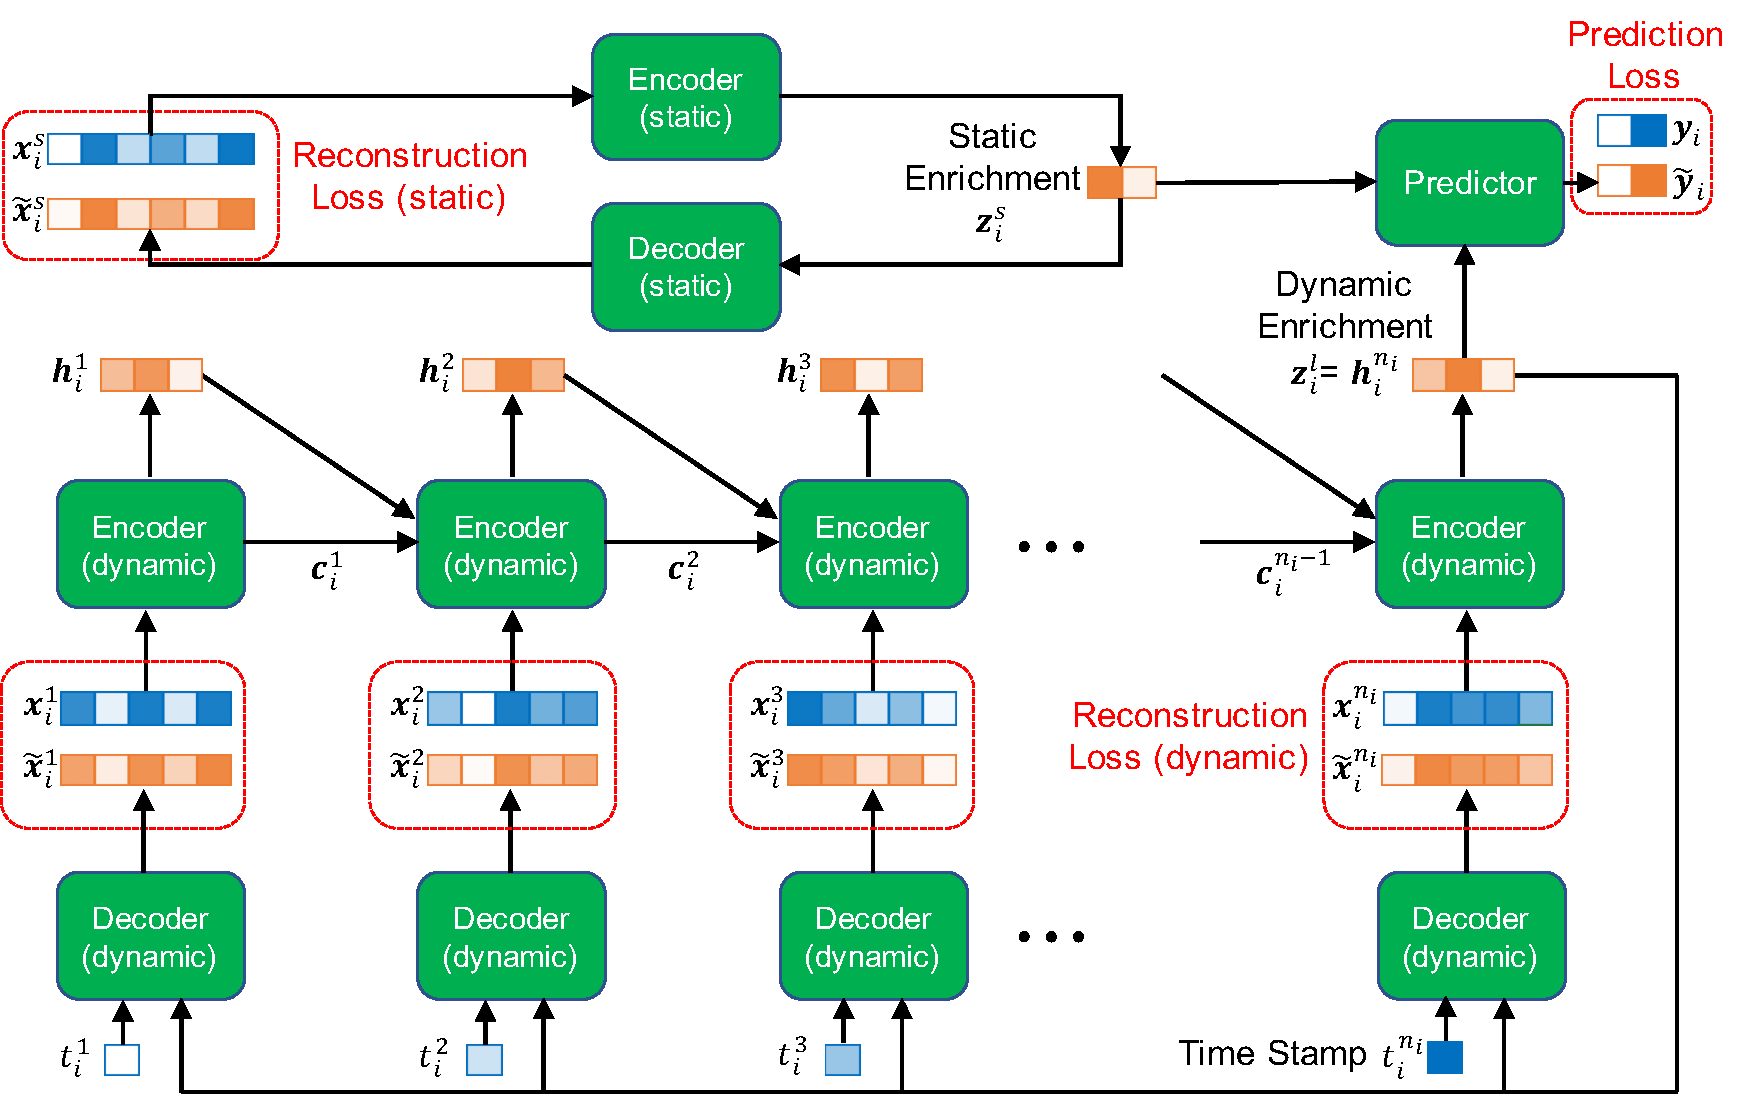
\includegraphics[width=\textwidth]{images/objective.pdf}
    \caption{An schematic illustration about loss function. Our semi-supervised learning autoencoder minimizes the reconstruction loss for the labeled or unlabeled samples, and prediction loss only for the labeled samples.} \label{fig: objective}
\end{figure}

\begin{figure}
    \centering
    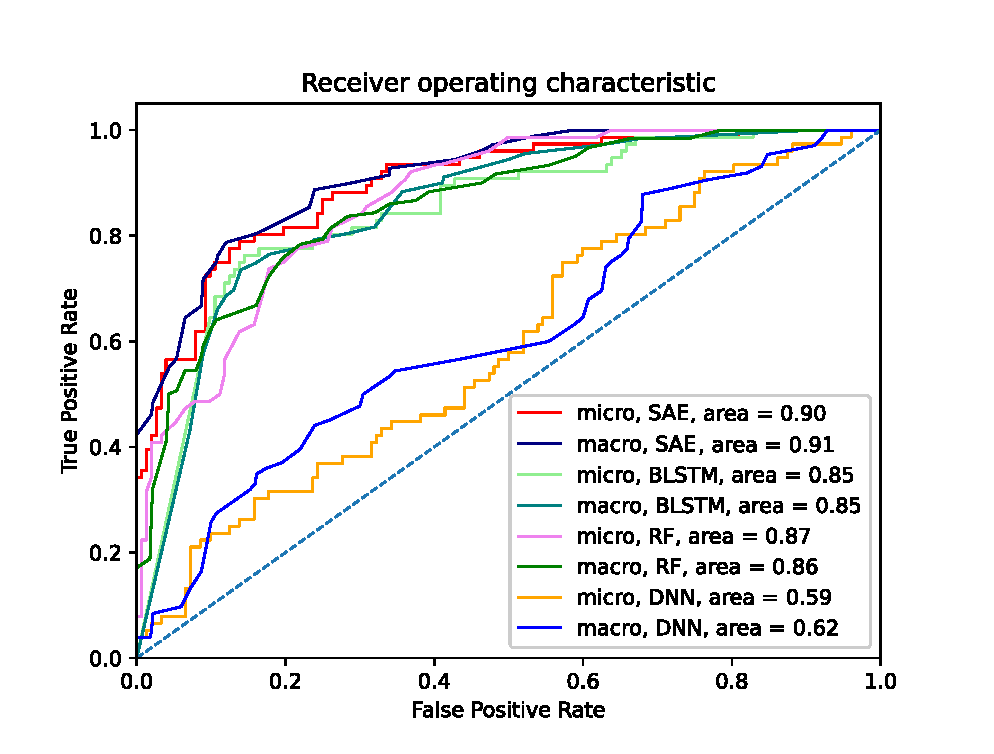
\includegraphics[width=0.89\textwidth]{images/roc_curve-p8.eps}
    \caption{Micro and macro receiver operating characteristic curves (ROC) averaged across the classes and their area under the curve (AUC). The proportion of training set is 80\% and the AUC shows SAE outperforms the other competing models.} \label{fig: roc_curve}
\end{figure}
\end{document}
